\documentclass[preprint,12pt]{elsarticle}

\usepackage[UTF8,scheme=plain]{ctex}
\usepackage[a4paper,margin=2.25cm]{geometry}
\usepackage{fontspec}
\usepackage{graphicx}
\usepackage{amsmath}
\usepackage{amssymb}
\usepackage{booktabs}
\usepackage{tabularx}
\usepackage{array}
\usepackage{threeparttable}
\usepackage{float}
\usepackage{placeins}
\usepackage{caption}
\usepackage{subcaption}
\usepackage{hyperref}
\hypersetup{hidelinks}

\setCJKmainfont[BoldFont=SimHei,ItalicFont=KaiTi]{SimSun}
\setCJKsansfont{SimHei}
\setmainfont{Times New Roman}
\setsansfont{Arial}
\linespread{1.12}
\emergencystretch=3em

\makeatletter
\setlength{\@fptop}{0pt}
\setlength{\@fpsep}{12pt}
\setlength{\@fpbot}{0pt plus 1fil}
\makeatother
\renewcommand{\topfraction}{0.95}
\renewcommand{\bottomfraction}{0.95}
\renewcommand{\textfraction}{0.06}
\renewcommand{\floatpagefraction}{0.80}
\setlength{\textfloatsep}{14pt plus 3pt minus 3pt}
\setlength{\floatsep}{12pt plus 3pt minus 3pt}

\journal{Spectrochimica Acta Part A / Talanta}
\graphicspath{{figures/}}

\newcommand{\cmone}{cm$^{-1}$}
\newcommand{\molA}{$10^{-4}$ M}
\newcommand{\molB}{$10^{-5}$ M}
\newcommand{\molC}{$10^{-6}$ M}
\newcolumntype{Y}{>{\raggedright\arraybackslash}X}
\newcolumntype{L}[1]{>{\raggedright\arraybackslash}p{#1}}
\newcommand{\figureplaceholder}[2]{%
  \fbox{%
    \begin{minipage}[c][#1][c]{0.94\textwidth}
      \centering\small #2
    \end{minipage}%
  }%
}

\captionsetup{font=small,labelfont=bf,labelsep=period}
\renewcommand{\figurename}{图}
\renewcommand{\tablename}{表}
\renewcommand{\abstractname}{摘要}
\renewcommand{\refname}{参考文献}
\abstracttitle{摘要}
\keywordtitle{关键词}
\makeatletter
\def\keywordname{关键词}
\makeatother

\begin{document}

\begin{frontmatter}

\title{三组分混合物 SERS 同步筛查与分级：竞争吸附诱导的孔雀石绿 1616 \texorpdfstring{cm$^{-1}$}{cm-1} 特征峰压制及可解释机器学习分析}

\author[inst1]{作者姓名}
\affiliation[inst1]{organization={辽宁石油化工大学人工智能与软件学院}, city={抚顺}, postcode={113001}, country={China}}

\begin{abstract}
多组分残留物的快速筛查是表面增强拉曼光谱（SERS）从单一标准品检测走向复杂样品应用的关键环节。本文以福美双（Thiram）、孔雀石绿（MG）和 4-巯基苯甲酸（4-MBA）三组分体系为对象，构建了基于柠檬酸银纳米颗粒胶体的 SERS-机器学习同步筛查流程，并同时设置目标物存在性识别与 \molA、\molB、\molC\ 三档离散浓度分级任务。混合物光谱显示出显著的共存干扰特征：MG 1616 \cmone\ 核心标志峰在 MG+MBA、MG+Thiram 和三元混合体系中的中位峰强比分别降至 0.355、0.206 和 0.129，其中 283/358 条三元混合谱低于同浓度档纯 MG 的 0.5 倍，表明竞争吸附可显著重塑混合物 SERS 峰强。13 类模型、6 种预处理策略和 6 个任务的系统比较显示，树集成模型在固定波数 SERS 指纹数据上表现稳定，各任务最优 macro-F1 达到 0.966--1.000。TreeSHAP 进一步将模型判别依据定位到化学相关谱区，22/29 个高贡献峰簇落在已知化学谱带上，覆盖 91.2\% 的总 SHAP 归因权重，说明模型主要依赖分子指纹峰和干扰敏感峰区完成判别。基于 SHAP 排序的谱区筛选显示，仅保留 10\% 高贡献波数（141/1401）时，六个任务的 macro-F1 仍全部高于 0.95。加标土壤基质筛查中，三个存在性任务获得 0.956--0.996 的 AUC，且 10 条空白/对照土壤光谱均被判定为阴性。该结果表明，三组分 SERS 混合物的关键难点不只是分类建模，而是共存吸附造成的目标峰压制；TreeSHAP 可将这一谱学干扰读出为化学相关判别峰区。
\end{abstract}

\begin{keyword}
表面增强拉曼光谱 \sep 三组分混合物 \sep 孔雀石绿 \sep 竞争吸附 \sep TreeSHAP \sep 机器学习 \sep 土壤基质筛查
\end{keyword}

\end{frontmatter}

\section{引言}

农药、染料和非法添加物的多组分共存使快速筛查比单一残留检测更接近真实样品场景。SERS 能在一次光谱采集中给出分子指纹信息，因此被用于果蔬、土壤和水体中污染物的快速识别\cite{HuApple,SMAMixture,SoilThiram}。在这类应用中，真正限制方法推广的往往不是单个分子的最低检出限，而是多个分子同时存在时的峰区重叠、信号压制和基质背景扰动。

已有研究已经证明 SERS 结合化学计量学可以处理二元混合残留。Hu 等将 SERS 与 self-modeling mixture analysis 结合，用于水果表面混合农药残留的快速无损检测\cite{SMAMixture}；Shi 等在苹果样品中使用 SERS 和多变量分析同时测定 pymetrozine 与 carbendazim，并指出混合溶液中两种农药的 SERS 强度显著低于单一溶液，竞争吸附会影响定量准确性\cite{HuApple}。Tian 等进一步将 DFT 计算与 SERS 实验结合，讨论 thiabendazole 与 pymetrozine 在银表面的竞争吸附，并用单组分与混合溶液的强度差异验证吸附竞争\cite{TianJFCA2025}；Altun 等也利用 SERS 强度变化敏感读出竞争性分子吸附过程\cite{CompetitiveAdsorption}。这些工作奠定了混合残留 SERS 分析基础，但主要围绕二元农药体系、连续定量或吸附模拟展开。

机器学习为多组分 SERS 光谱提供了全谱判别能力，但模型本身仍需要谱学解释支撑。光谱解释方法已经用于 Raman、SERS 和其他光谱模型中，以定位重要波数并将模型判别与化学峰带联系起来\cite{SHAPLIME,SHAPSegmentation,XAIDLSERS,ZnOSHAP}。不过，在三组分 SERS 混合物中，将竞争吸附诱导的特征峰压制、同步筛查/分级模型和 TreeSHAP 化学归因放在同一研究设计中结合报道的工作仍然有限。尤其是当目标峰被共存组分系统性压制时，模型究竟读取目标物自身指纹，还是读取共存干扰留下的谱学线索，是三组分筛查中必须回答的问题。

基于上述问题，本文以 Thiram、MG 和 4-MBA 为三组分模型体系，采用柠檬酸 AgNPs 胶体采集纯组分、二元和三元混合物 SERS 谱，并建立机器学习筛查/分级模型。本文首先构建 \molA、\molB\ 和 \molC\ 三档离散浓度下的存在性筛查和分级任务，然后比较 13 类模型与 6 种预处理策略的任务性能；在此基础上，重点分析 MG 1616 \cmone\ 特征峰在二元和三元共存条件下的压制，并利用 TreeSHAP 将模型判别谱区映射到已知化学峰带。最后，本文评估 SHAP 引导的 10\% 波数保留策略，并在加标土壤基质中验证存在性筛查表现。实验与建模设计如图~\ref{fig:workflow} 所示。

\begin{figure}[!htbp]
  \centering
  \IfFileExists{fig1_workflow.pdf}{%
    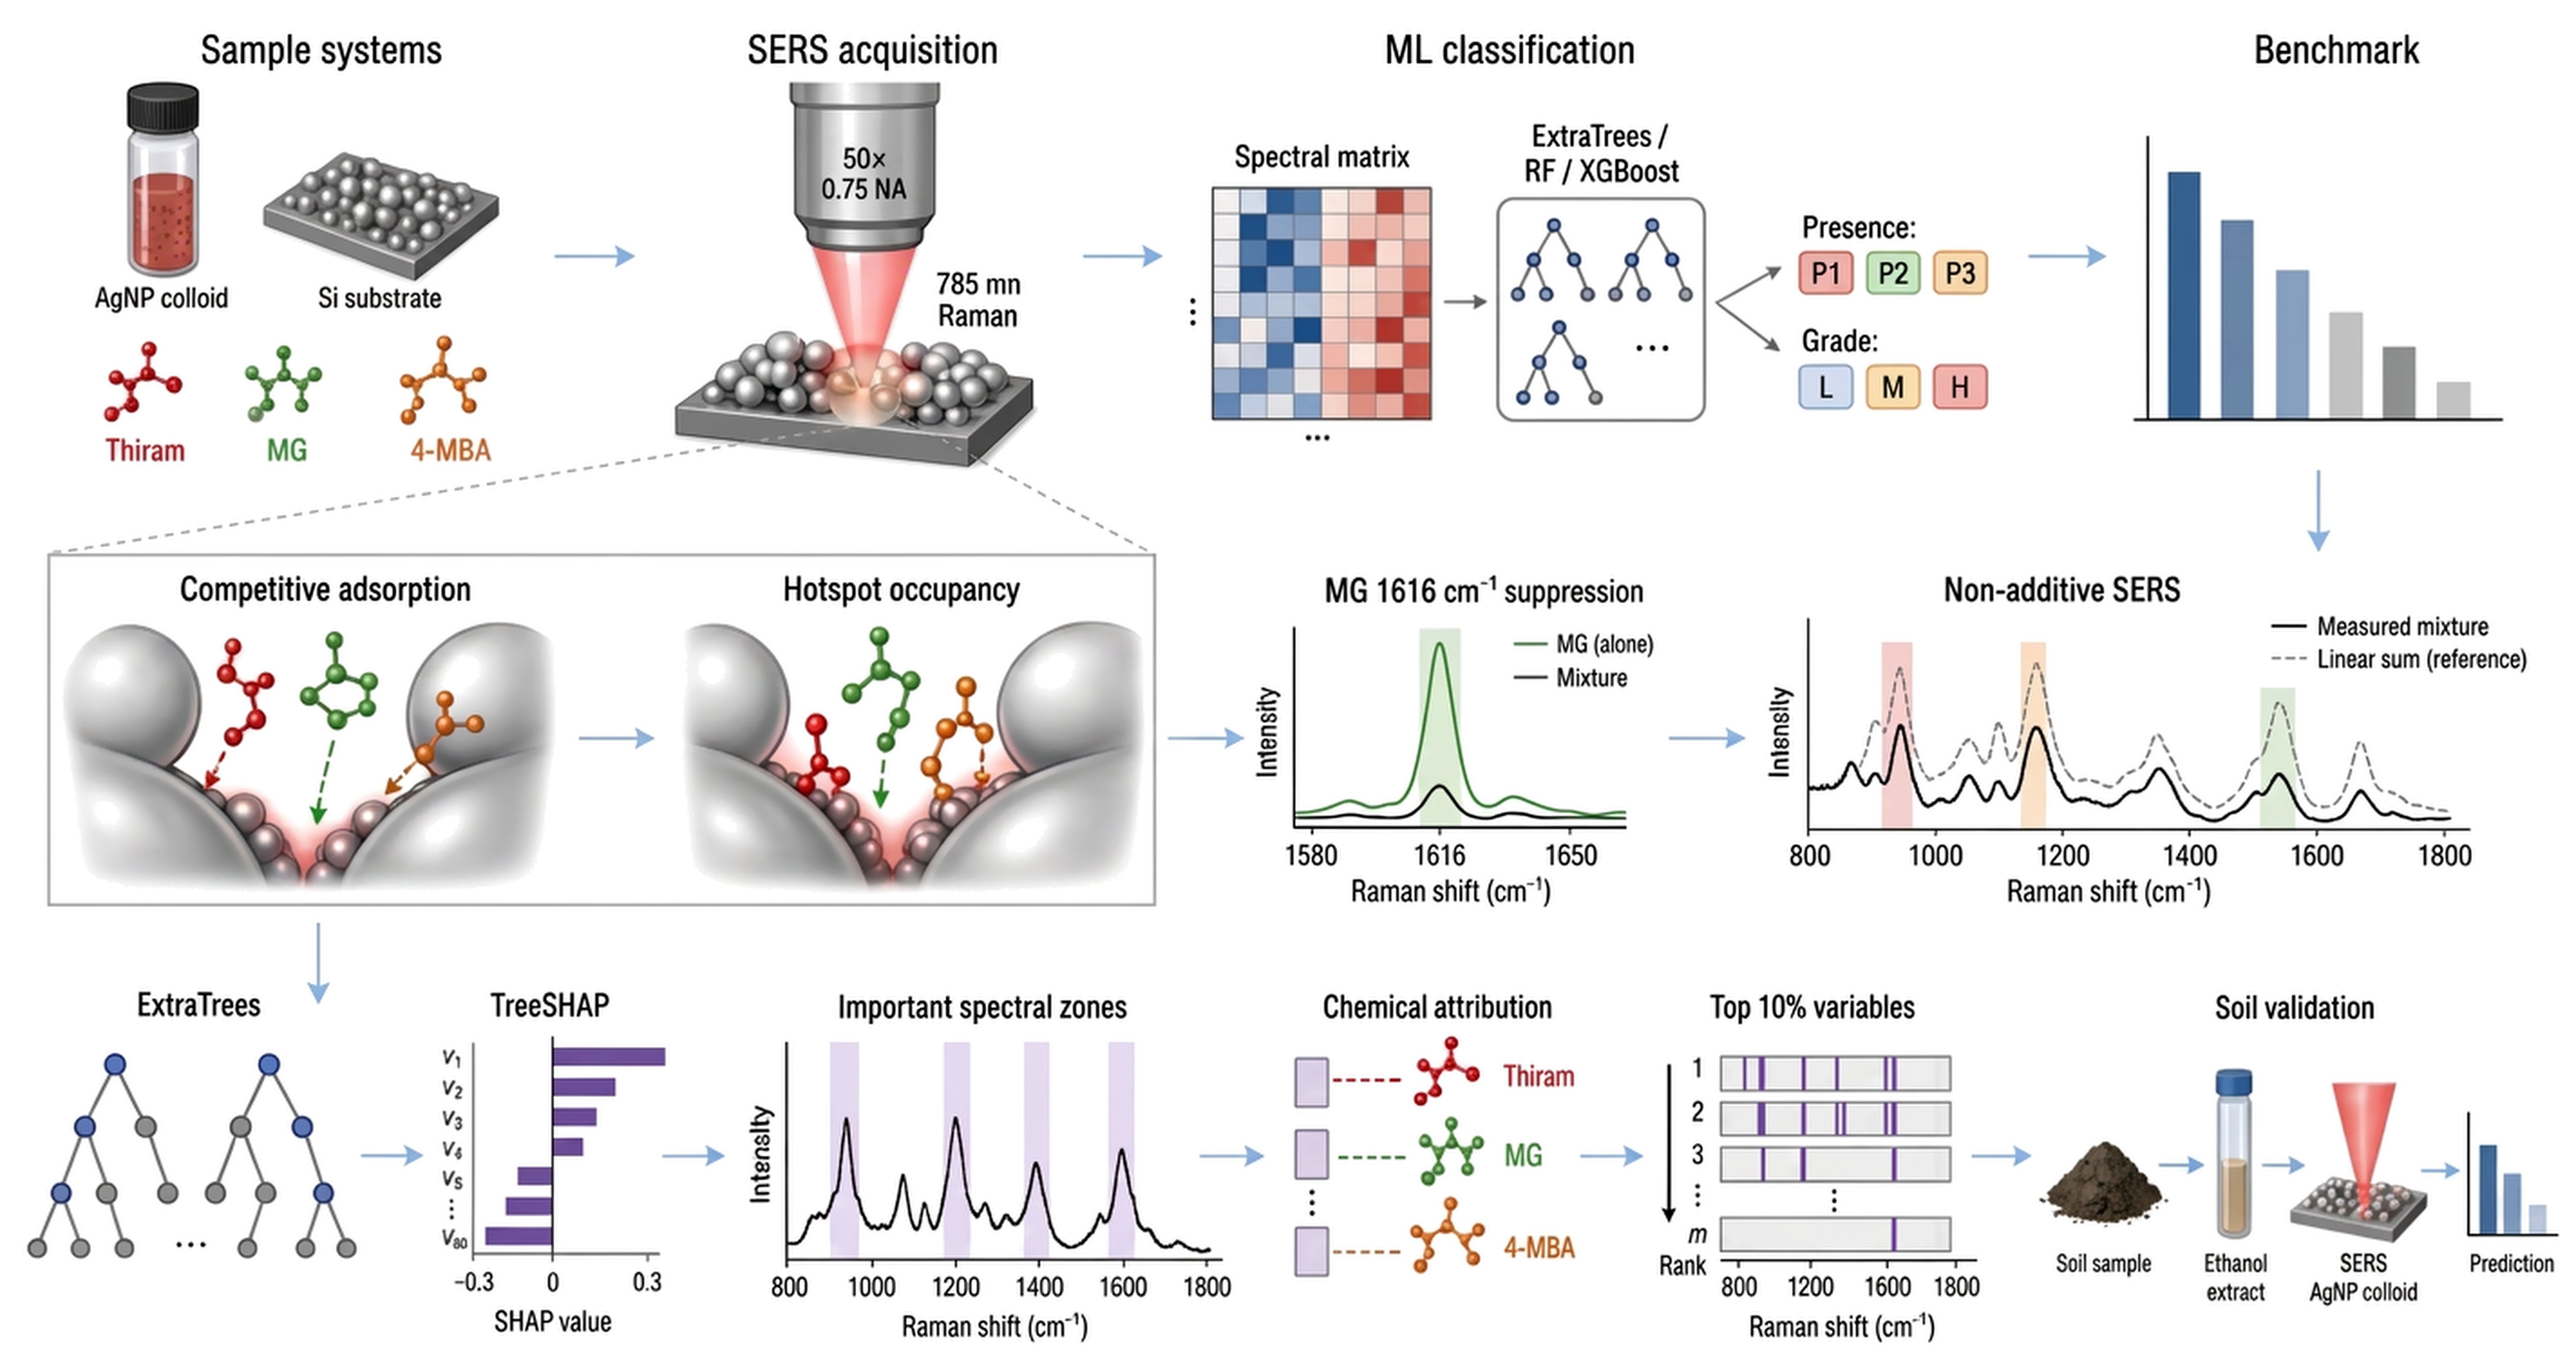
\includegraphics[width=0.96\textwidth]{fig1_workflow.pdf}%
  }{%
    \figureplaceholder{6.4cm}{\textbf{图 1 研究流程示意图}\\[0.6em]
    柠檬酸 AgNP 胶体基底、Thiram/MG/4-MBA 三组分样品设计、SERS 光谱采集、同步筛查与分级、MG 1616 \cmone\ 峰压制、TreeSHAP 归因、紧凑谱区筛选和加标土壤基质验证。}%
  }
  \caption{基于柠檬酸 AgNPs 胶体的三组分 SERS-机器学习分析流程。}
  \label{fig:workflow}
\end{figure}
\FloatBarrier

\section{材料与方法}

\subsection{试剂、仪器与 AgNPs 胶体制备}

Thiram、MG、4-MBA、硝酸银和柠檬酸钠均为分析纯或以上等级。Thiram（97\%）和 AgNO$_3$（99\%）购自 Innochem Technology Co., Ltd.，柠檬酸钠（99\%）购自 Sinopharm Chemical Reagent Co., Ltd.，4-MBA（90\%）和 MG（AR）购自 Shanghai Aladdin Biochemical Technology Co., Ltd.。SERS 光谱由便携式拉曼光谱仪采集（BWS465-785S, B\&W-Tek, USA），激发波长为 785 nm，仪器采集范围为 110--2000 \cmone。建模和图谱分析使用 400--1800 \cmone\ 指纹区。AgNPs 胶体的光学吸收由 Agilent Cary 系列 UV-Vis-NIR 分光光度计记录，纳米颗粒形貌由电子显微镜表征。

AgNPs 采用柠檬酸钠还原法制备，该路线也是银胶体 SERS 基底中常用的快速制备方法\cite{TianJFCA2025}。玻璃器皿先经王水（HNO$_3$:HCl = 1:3, v/v）清洗，再用超纯水充分冲洗。将 0.0342 g AgNO$_3$ 溶于 200 mL 超纯水，在 250 r/min 搅拌下加热至回流并保持 25 min；随后快速加入 4 mL 0.01 mol/L 柠檬酸钠溶液，并在 100 $^\circ$C 下继续反应 20 min。反应液自然冷却至室温后，以 1500 r/min 离心 5 min，收集下层浊色胶体用于 SERS 检测。

\subsection{三组分样品设计与加标土壤样品制备}

Thiram、MG 和 4-MBA 分别配制为 \molA、\molB\ 和 \molC\ 三个离散浓度档。纯组分、二元混合物和三元混合物按目标配方现配，用于建立三组分 SERS 指纹数据集。每个目标物同时参与两类任务：P1/P2/P3 用于判断 Thiram、MG 和 4-MBA 是否存在，G1/G2/G3 用于判断目标物处于 \molA、\molB\ 或 \molC\ 三个浓度档中的哪一档。该任务设计对应快速筛查中常见的“有无判断 + 离散风险档分级”模式。

土壤基质样品参照 Dong 等土壤 SERS-机器学习工作中的加标-萃取流程处理\cite{SoilThiram}。土壤样品经干燥、除杂、研磨和均质化后称取约 1.0 g，加入 Thiram、MG 和 4-MBA 混合标准溶液并混匀，自然干燥后得到加标土壤样品；未加标土壤按相同流程处理作为空白/对照样品。随后加入约 1 mL 乙醇萃取土壤中的目标物，涡旋振荡约 1 min 后静置分层，取上清液用于 AgNPs 辅助 SERS 采集。共采集 79 条加标土壤 SERS 光谱和 10 条土壤空白/对照光谱，用于评价模型在土壤基质中的存在性筛查性能。

\subsection{SERS 光谱采集与预处理}

标准品和混合物样品采用滴加式 SERS 采集方式。每次取 2 $\mu$L 待测溶液滴加于商业硅胶板或等效惰性载体表面，随后加入 2 $\mu$L AgNPs 胶体形成检测点，并在不同采样位置采集重复光谱；土壤基质样品经萃取后按相同 AgNPs 辅助流程采集。每条光谱经统一波数校准后截取 400--1800 \cmone\ 区间，共包含 1401 个波数点。

本文比较原始谱与 p1--p5 共 6 种输入形式。其中 p1 为宇宙射线校正、Savitzky--Golay 平滑、ALS 基线校正和 SNV；p2 为平滑、ALS 基线校正、一阶导数和 SNV；p3 为 ALS 基线校正和向量归一化；p4 为宇宙射线校正、平滑和 ALS 基线校正；p5 为宇宙射线校正、平滑、ALS 基线校正、二阶导数和 SNV。系统模型比较、TreeSHAP 归因、谱区筛选和土壤基质验证采用 p1 作为主输入；MG 1616 \cmone\ 峰压制分析采用未归一化的 p4 光谱，以保留峰强变化信息。为量化共存组分对 MG 特征峰的压制，定义同一 MG 浓度档下混合谱与纯 MG 参考谱的峰强比：
\begin{equation}
R_{c}^{1616}=\frac{I_{mix,c}^{1616}}{I_{pure,c}^{1616}},
\end{equation}
其中 $I_{mix,c}^{1616}$ 和 $I_{pure,c}^{1616}$ 分别表示浓度档 $c$ 下混合物和纯 MG 光谱中 1616 \cmone\ 峰强。正文以各共存条件下 $R_{c}^{1616}$ 的中位数作为峰压制程度的主要表征。

\subsection{机器学习建模与评价指标}

本文比较 13 类模型，包括 Random Forest、ExtraTrees、HistGradientBoosting、XGBoost、SVM、KNN、PLS-DA、LDA、1D-CNN、1D-ResNet、Spectrum-KAN、KAN-CNN 和 RamanNet-Lite。每种模型与 6 种预处理策略、6 个任务组合，形成 468 个模型-预处理-任务实验点。模型性能采用分层五折交叉验证评估，主要指标为 macro-F1，balanced accuracy 和 accuracy 作为辅助指标。

对于第 $k$ 个类别，precision、recall 和 F1 定义为：
\begin{equation}
P_k=\frac{TP_k}{TP_k+FP_k}, \quad
R_k=\frac{TP_k}{TP_k+FN_k}, \quad
F1_k=\frac{2P_kR_k}{P_k+R_k}.
\end{equation}
多分类任务的 macro-F1 和 balanced accuracy 分别计算为：
\begin{equation}
\mathrm{Macro\text{-}F1}=\frac{1}{K}\sum_{k=1}^{K}F1_k, \quad
\mathrm{BA}=\frac{1}{K}\sum_{k=1}^{K}\frac{TP_k}{TP_k+FN_k}.
\end{equation}
土壤存在性筛查任务同时报告 ROC-AUC、空白特异性和标签置换检验结果。所有数据整理和统计分析在 Python 环境中完成，传统机器学习模型主要基于 scikit-learn 和 XGBoost 实现，深度学习对照模型基于 PyTorch 实现，TreeSHAP 归因使用 SHAP 软件包计算。

\subsection{TreeSHAP 归因与紧凑谱区筛选}

综合模型比较结果，ExtraTrees/p1 被选为 TreeSHAP 归因、谱区筛选和土壤基质筛查的主模型。对 P1/P2/P3/G1/G2/G3 六个任务分别计算每个波数的平均绝对 SHAP 贡献：
\begin{equation}
S_j^{(t)}=\frac{1}{n}\sum_{i=1}^{n}\left|\phi_{ij}^{(t)}\right|,
\end{equation}
其中 $S_j^{(t)}$ 表示任务 $t$ 下第 $j$ 个波数的贡献强度，$\phi_{ij}^{(t)}$ 为第 $i$ 条光谱在该波数处的 SHAP 值。高贡献波数进一步聚类为峰簇，并根据 Thiram、MG 和 4-MBA 的已知 SERS/Raman 特征峰及本实验纯谱峰库进行化学归属。化学峰带归属一致性按贡献权重计算：
\begin{equation}
M=\frac{\sum_{j\in C_{matched}}S_j}{\sum_{j\in C_{all}}S_j},
\end{equation}
其中 $C_{matched}$ 表示落在已知化学谱带上的高贡献峰簇，$C_{all}$ 表示全部高贡献峰簇。

为将模型解释转化为紧凑谱区筛查策略，本文按 $S_j^{(t)}$ 对 1401 个波数排序，仅保留前 $q$ 比例的高贡献波数，其余波数置零：
\begin{equation}
x'_j=x_j\cdot \mathbb{I}\left(j\in \mathrm{Top}_{q}(S^{(t)})\right).
\end{equation}
随后在相同五折设置下重训 ExtraTrees，并比较不同保留比例下的筛查/分级性能。

\section{结果与讨论}

\subsection{纯组分 SERS 指纹与检测重复性}

纯组分重复光谱为三组分筛查提供了分子指纹基础（图~\ref{fig:repeatability}）。Thiram、MG 和 4-MBA 均呈现清晰且可重复的特征峰。代表峰面积 RSD 分别为 Thiram 1382 \cmone\ 的 10.2\%、MG 1616 \cmone\ 的 6.0\% 和 4-MBA 1080 \cmone\ 的 2.6\%，与已发表 SERS 方法中用于支撑基底重复性的 RSD 水平相当\cite{HuApple,TianJFCA2025,SoilThiram}。这一重复性水平构成了后续比较混合体系与纯 MG 参考谱中 1616 \cmone\ 峰强的稳定基线。

\begin{figure}[!htbp]
  \centering
  
\includegraphics[width=0.96\textwidth]{fig2_quality_panels.pdf}
  \caption{纯组分重复 SERS 光谱与代表峰面积重复性。a，Thiram、MG 和 4-MBA 在 \molA\ 下的重复光谱；b，代表峰面积 RSD。}
  \label{fig:repeatability}
\end{figure}
\FloatBarrier

三种分析物的纯组分 SERS 谱进一步显示出可用于识别和归属的典型峰带（图~\ref{fig:spectra}）。Thiram 在 560、930、1380 和 1510 \cmone\ 附近具有代表性峰；MG 在 1172、1220、1394 和 1616 \cmone\ 附近呈现特征指纹；4-MBA 在 1078 和 1590 \cmone\ 附近具有稳定峰带。表~\ref{tab:peaks} 总结了正文使用的核心峰归属。MG 1616 \cmone\ 位于相对干净的高波数区，可作为 MG 信号变化的核心标志峰；1172 和 1394 \cmone\ 虽与 MG 相关，但处于更容易发生邻近峰干扰和峰包络重塑的窗口，因此在本文中作为 MG 相关重叠敏感峰区处理。

\begin{figure}[!htbp]
  \centering
  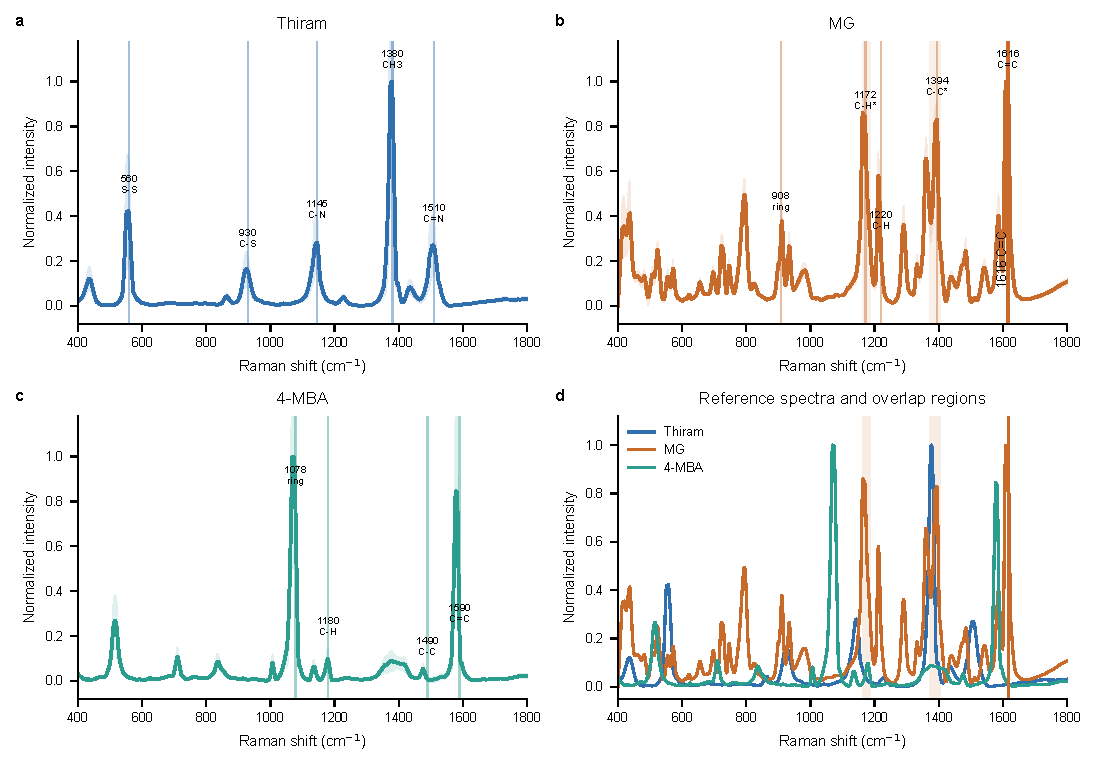
\includegraphics[width=0.96\textwidth]{fig3_spectra.pdf}
  \caption{Thiram、MG 和 4-MBA 的纯组分 SERS 谱及特征峰归属。MG 1616 \cmone\ 作为核心标志峰用于后续压制分析，1172/1394 \cmone\ 作为 MG 相关重叠敏感峰区。}
  \label{fig:spectra}
\end{figure}

\begin{table}[!htbp]
\centering
\caption{Thiram、MG 和 4-MBA 的正文核心 SERS 峰及振动归属。}
\label{tab:peaks}
\small
\begin{tabularx}{\textwidth}{L{1.55cm}L{1.55cm}Y L{3.35cm}}
\toprule
分析物 & 位移 (\cmone) & 振动归属 & 正文用途 \\
\midrule
Thiram & 560 & S--S 伸缩/骨架振动 & Thiram 指纹峰 \\
Thiram & 930 & C--S 对称伸缩 & Thiram 指纹峰 \\
Thiram & 1380 & CH$_3$ 变形/C--N 相关振动 & Thiram 主要峰，重叠敏感区 \\
Thiram & 1510 & C=N/C--N 相关振动 & Thiram 指纹峰 \\
MG & 1172 & C--H 面内弯曲 & MG 相关重叠敏感峰区 \\
MG & 1220 & C--H 面内弯曲 & MG 指纹峰 \\
MG & 1394 & 芳环 C--C/C--N 相关振动 & MG 相关重叠敏感峰区 \\
MG & 1616 & 芳环 C=C 伸缩 & MG 压制分析核心标志峰 \\
4-MBA & 1078 & 环呼吸/C--S 相关振动 & 4-MBA 指纹峰 \\
4-MBA & 1590 & 芳环 C=C 伸缩 & 4-MBA 指纹峰 \\
\bottomrule
\end{tabularx}
\end{table}
\FloatBarrier

\subsection{系统模型比较展示三组分同步筛查与分级性能}

13 模型 $\times$ 6 预处理 $\times$ 6 任务的系统模型比较显示，三组分 SERS 指纹能够支撑存在性筛查和三档离散浓度分级（图~\ref{fig:modelcompare}）。六个任务的各任务最优 macro-F1 均处于较高水平：P1 Thiram 存在性筛查为 0.996$\pm$0.006，P2 MG 存在性筛查为 0.985$\pm$0.009，P3 4-MBA 存在性筛查为 0.994$\pm$0.006；G1 Thiram 分级为 1.000$\pm$0.000，G2 MG 分级为 0.966$\pm$0.009，G3 4-MBA 分级为 0.981$\pm$0.007（表~\ref{tab:modelcompare}）。这些数值表明，固定波数 SERS 指纹不仅可用于三种目标物的有无判断，也可区分 \molA、\molB\ 和 \molC\ 三个离散浓度档。

\begin{figure}[!htbp]
  \centering
  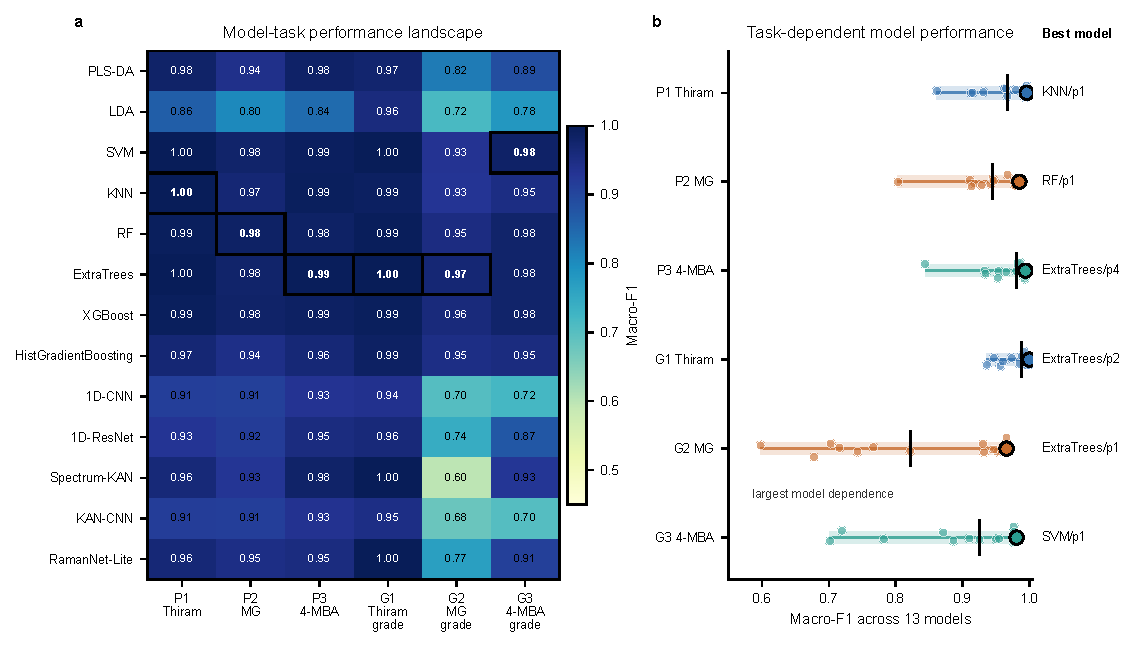
\includegraphics[width=0.96\textwidth]{fig4_benchmark_heatmap.pdf}
  \caption{13 类模型在六个筛查/分级任务中的系统比较。树集成模型表现出稳定的多任务筛查性能，G2/MG 分级任务呈现更宽的跨模型性能分布。}
  \label{fig:modelcompare}
\end{figure}

\begin{table}[!htbp]
\centering
\caption{系统模型比较中六个任务的最优性能。}
\label{tab:modelcompare}
\scriptsize
\resizebox{\textwidth}{!}{%
\begin{tabular}{llllll}
\toprule
任务 & 最优模型 & 预处理 & Macro-F1 & Balanced accuracy & Accuracy \\
\midrule
P1 Thiram 存在性筛查 & KNN & p1 & 0.996$\pm$0.006 & 0.998$\pm$0.003 & 0.997$\pm$0.005 \\
P2 MG 存在性筛查 & RF & p1 & 0.985$\pm$0.009 & 0.987$\pm$0.009 & 0.988$\pm$0.007 \\
P3 4-MBA 存在性筛查 & ExtraTrees & p4 & 0.994$\pm$0.006 & 0.991$\pm$0.010 & 0.996$\pm$0.005 \\
G1 Thiram 分级 & ExtraTrees & p2 & 1.000$\pm$0.000 & 1.000$\pm$0.000 & 1.000$\pm$0.000 \\
G2 MG 分级 & ExtraTrees & p1 & 0.966$\pm$0.009 & 0.967$\pm$0.009 & 0.966$\pm$0.009 \\
G3 4-MBA 分级 & SVM & p1 & 0.981$\pm$0.007 & 0.981$\pm$0.006 & 0.981$\pm$0.007 \\
\bottomrule
\end{tabular}}
\end{table}
\FloatBarrier

模型层面的比较进一步表明，树集成模型与固定波数 SERS 指纹具有较好的适配性。跨任务和跨预处理平均后，ExtraTrees、XGBoost 和 Random Forest 的平均 macro-F1 分别达到 0.971、0.969 和 0.966，领先于本研究测试的深度学习基线。Grinsztajn 等在典型表格数据上观察到树模型相对于深度学习的稳定优势\cite{Grinsztajn2022}；本文的固定波数 SERS 光谱同样具有表格化输入、高维但有效峰区稀疏的特点。ExtraTrees/p1 在多任务上表现均衡，因此被用于后续 TreeSHAP 归因、谱区筛选和土壤基质筛查。

不同任务对模型选择的敏感性揭示了 MG 分级的特殊谱学背景。G2/MG 分级在最佳模型下可达到 0.966$\pm$0.009，但其跨模型分布范围更宽，部分深度学习和 KAN 模型在该任务上的表现明显低于其他任务。这一现象指向混合谱强度变化和干扰峰区处理方式的差异，并引出下一节对 MG 1616 \cmone\ 特征峰压制的分析。

\subsection[三组分共存显著压制 MG 1616 cm-1 特征峰]{三组分共存显著压制 MG 1616 \cmone\ 特征峰}

混合物光谱分析表明，MG 的核心标志峰在共存体系中发生显著衰减（图~\ref{fig:mgsuppression}）。以同一 MG 浓度档纯 MG 光谱作为参考，MG+MBA、MG+Thiram 和三元混合体系中 1616 \cmone\ 峰的中位峰强比分别为 0.355、0.206 和 0.129。也就是说，在三元体系中，MG 1616 \cmone\ 的中位信号仅保留同浓度档纯 MG 的约 12.9\%。逐谱统计进一步显示，MG+MBA 中 86/128 条光谱、MG+Thiram 中 65/100 条光谱、三元体系中 283/358 条光谱的 1616 \cmone\ 强度低于同浓度档纯 MG 的 0.5 倍。

\begin{figure}[!htbp]
  \centering
  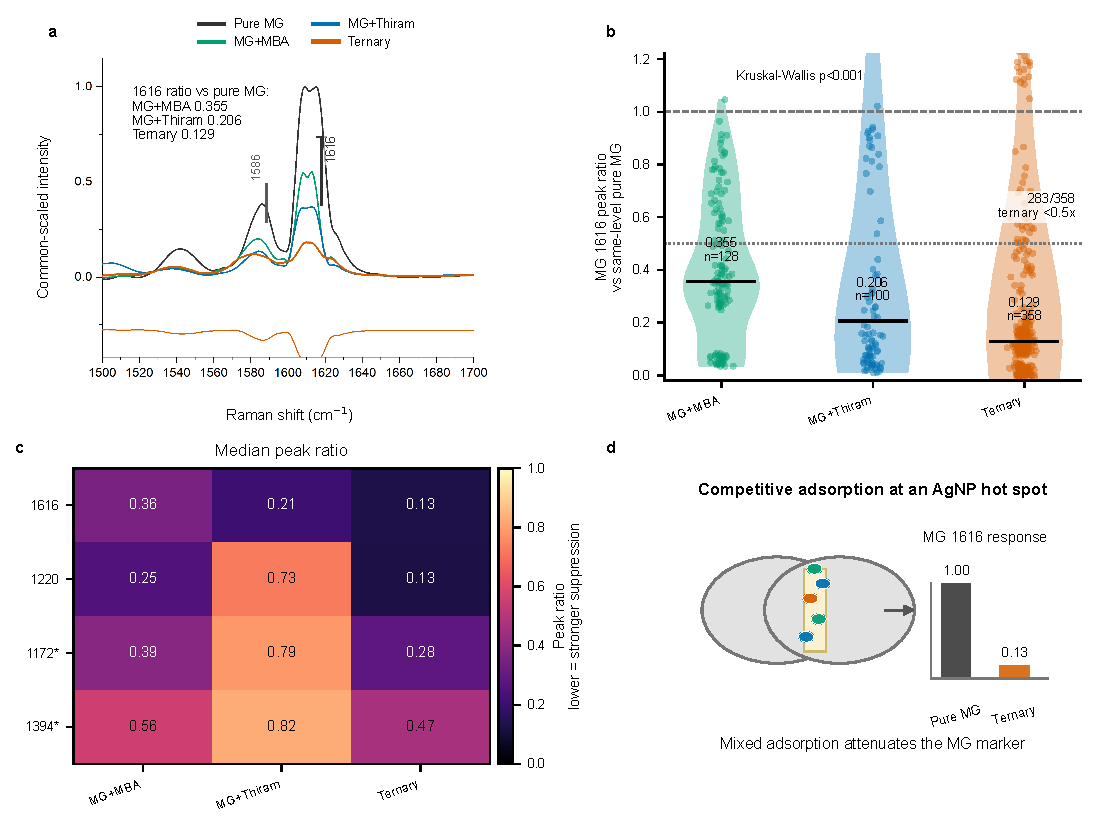
\includegraphics[width=0.96\textwidth]{fig5_mg_suppression.pdf}
  \caption{共存组分显著压制 MG 1616 \cmone\ 核心标志峰。二元和三元共存使 MG 1616 \cmone\ 峰强分别降至同浓度档纯 MG 参考的 0.355、0.206 和 0.129，揭示竞争吸附诱导的混合物谱峰干扰。}
  \label{fig:mgsuppression}
\end{figure}
\FloatBarrier

Shi 等在 pymetrozine/carbendazim 混合溶液中观察到两种农药的特征峰强均低于单一溶液，并将其归因于 Au@AgNPs 表面的竞争吸附\cite{HuApple}；Tian 等也报道了混合吸附会削弱 thiabendazole 与 pymetrozine 的理论和实验 SERS 强度\cite{TianJFCA2025}。与这些二元体系不同，本文中 MG 1616 \cmone\ 的中位残余强度从 MG+MBA 的 35.5\% 和 MG+Thiram 的 20.6\% 进一步降至三元体系的 12.9\%，显示三组分共存带来更强的目标峰压制。Thiram 和 4-MBA 均可通过含硫基团或较强表面相互作用占据银纳米颗粒热点区域，降低 MG 的有效吸附和局域增强机会。1172、1220 和 1394 \cmone\ 等 MG 相关峰区也呈现不同程度的衰减或包络变化，其中 1172/1394 \cmone\ 作为重叠敏感区，进一步说明混合谱不能被简化为单一峰强规则。

该谱学发现使 G2/MG 分级任务的模型敏感性具有明确的化学解释。MG 存在性任务主要判断是否存在 MG 指纹，而 MG 分级任务需要区分三个离散浓度档；当 1616 \cmone\ 核心标志峰在共存体系中被显著压制时，不同浓度档之间的强度差异被共存背景重新塑形，模型必须同时利用 MG 相关峰、重叠敏感峰区和共存组分带来的干扰线索。因此，G2 是三组分 SERS 混合物中竞争吸附干扰最直观的读出窗口。

\subsection{TreeSHAP 将模型判别定位到化学相关峰区}

为进一步说明模型判别依据，本文对 ExtraTrees/p1 进行 TreeSHAP 归因，并将高贡献波数聚类为峰簇（图~\ref{fig:shap}）。22/29 个 SHAP 高贡献峰簇落在已知化学谱带上，覆盖 91.2\% 的总 SHAP 归因权重。模型权重主要集中在 Thiram、MG 和 4-MBA 的分子指纹峰，以及由共存体系引起的干扰敏感谱区。

\begin{figure}[!htbp]
  \centering
  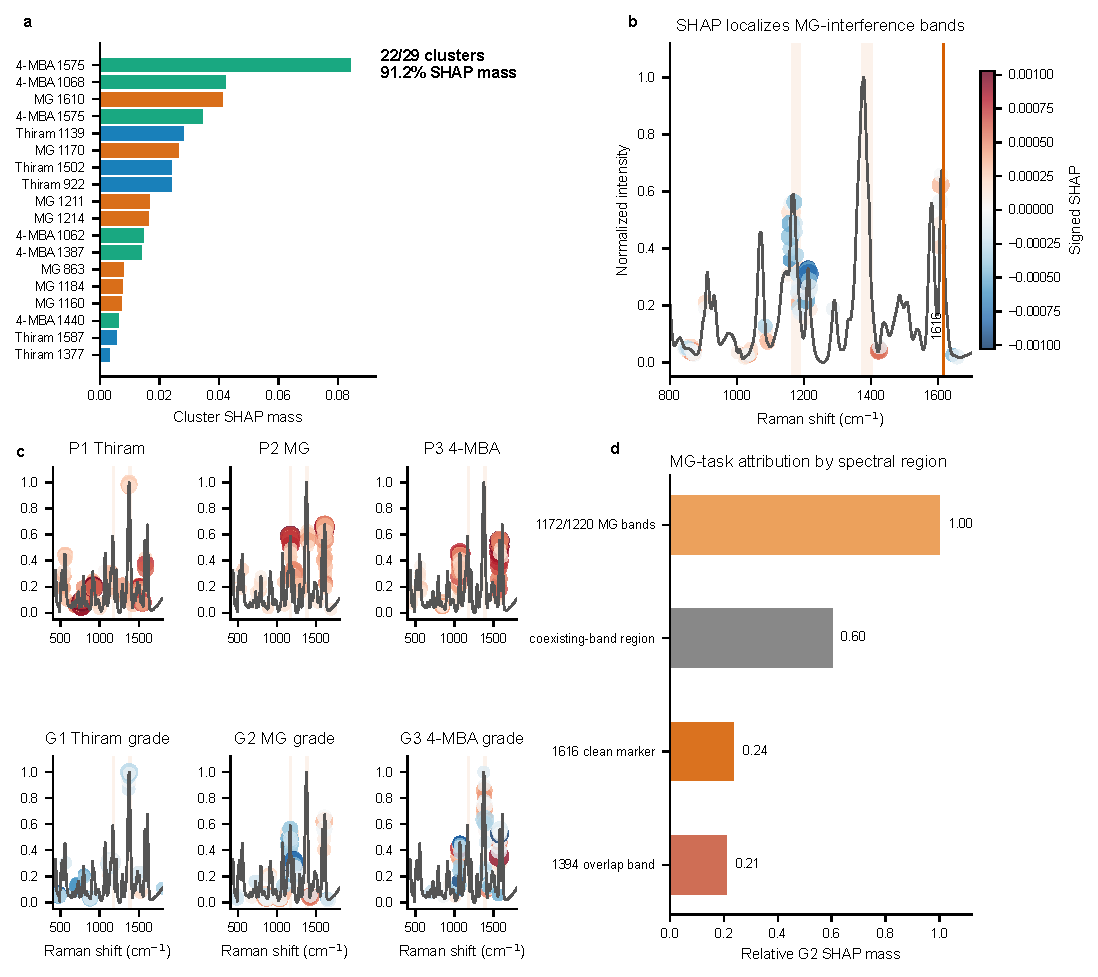
\includegraphics[width=0.96\textwidth]{fig6_shap_attribution.pdf}
  \caption{TreeSHAP 将模型判别谱区定位到已知化学峰带。共 22/29 个 SHAP 高贡献峰簇落在已知化学谱带上，覆盖 91.2\% 的总 SHAP 归因权重。}
  \label{fig:shap}
\end{figure}
\FloatBarrier

P2/MG 存在性筛查的高贡献区域集中在 MG 1172、1394 和 1616 \cmone\ 附近；P3/4-MBA 存在性筛查的高贡献区域集中在 1078 和 1590 \cmone\ 附近；G1/Thiram 分级主要利用 Thiram 1145、1380 和 1510 \cmone\ 附近信息。对于 G2/MG 分级，模型除使用 MG 1220 和 1616 \cmone\ 附近信息外，还捕获了 Thiram 相关干扰带。这种跨组分干扰归因说明，模型在处理 MG 分级时同时利用了 MG 自身峰和共存组分对混合谱造成的干扰线索。

TreeSHAP 归因将图~\ref{fig:mgsuppression} 中观察到的 MG 1616 \cmone\ 压制和峰包络重塑，与图~\ref{fig:modelcompare} 中模型实际使用的谱区连接起来。模型的主要贡献区集中在具有明确谱学意义的峰带和干扰敏感窗口，使三组分混合物的分类结果能够回到具体光谱特征中解释。

\subsection{SHAP 引导谱区筛选实现紧凑谱区筛查}

按每个任务的 mean $|\mathrm{SHAP}|$ 排序后，仅保留前 10\% 波数，即 141/1401 个光谱变量，并用置零后的光谱重训 ExtraTrees。六个任务的 macro-F1 仍全部高于 0.95：P1、P2、P3、G1、G2 和 G3 分别为 0.986、0.969、0.982、0.979、0.953 和 0.974（图~\ref{fig:fs}）。与全谱输入相比，10\% 高贡献波数已经保留了足够的判别信息。

\begin{figure}[!htbp]
  \centering
  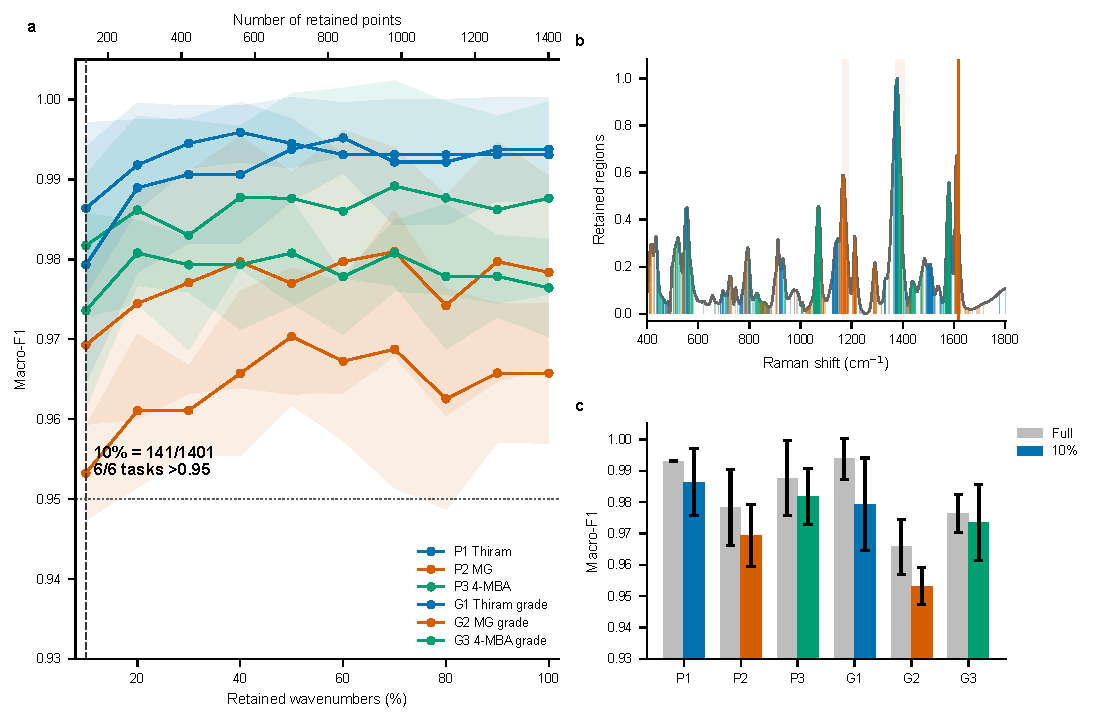
\includegraphics[width=0.96\textwidth]{fig7_feature_elimination.pdf}
  \caption{SHAP 引导谱区筛选在 10\% 光谱变量下保持筛查性能。仅使用 141/1401 个高贡献波数时，六个任务的 macro-F1 均保持在 0.95 以上。}
  \label{fig:fs}
\end{figure}
\FloatBarrier

10\% 保留比例对应 141 个波数点，显著低于原始 1401 点全谱输入，但仍保留峰形邻域信息，可覆盖峰位偏移、峰宽变化和混合物峰包络重塑。与只选取少数孤立峰相比，SHAP 保留谱区包含目标分子指纹峰、共吸附相关峰区和干扰敏感窗口，更适合三组分混合物筛查。

\subsection{加标土壤基质筛查验证}

加标土壤基质进一步验证了该方法在复杂背景中的存在性筛查能力（图~\ref{fig:soil}）。Thiram、MG 和 4-MBA 三个存在性筛查任务的 AUC 分别达到 0.996$\pm$0.008、0.956$\pm$0.052 和 0.976$\pm$0.034；对应 macro-F1 分别为 0.887$\pm$0.087、0.811$\pm$0.127 和 0.919$\pm$0.085（表~\ref{tab:soil}）。标签置换检验显示三个任务的观测 AUC 均显著高于随机置换分布，$p<10^{-4}$。

\begin{figure}[!htbp]
  \centering
  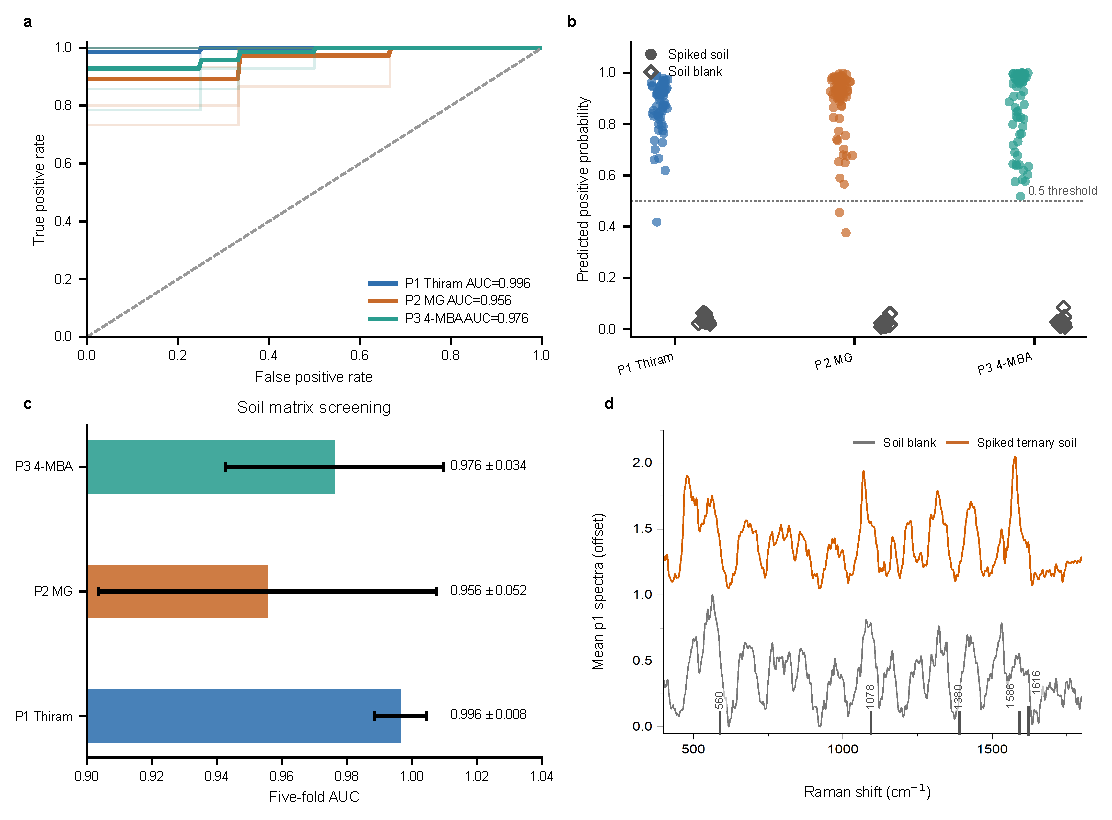
\includegraphics[width=0.96\textwidth]{fig8_soil_screening.pdf}
  \caption{Thiram、MG 和 4-MBA 存在性任务的加标土壤基质筛查验证。ROC 分析、空白特异性和置换检验给出土壤基质中的筛查性能。}
  \label{fig:soil}
\end{figure}

\begin{table}[!htbp]
\centering
\caption{三个存在性任务的加标土壤基质筛查指标。}
\label{tab:soil}
\scriptsize
\resizebox{\textwidth}{!}{%
\begin{tabular}{llllllll}
\toprule
任务 & 加标光谱 & 空白/对照光谱 & 总光谱数 & AUC & Macro-F1 & Balanced accuracy & 空白特异性 \\
\midrule
P1 Thiram & 79 & 10 & 89 & 0.996$\pm$0.008 & 0.887$\pm$0.087 & 0.868$\pm$0.117 & 1.000 \\
P2 MG & 79 & 10 & 89 & 0.956$\pm$0.052 & 0.811$\pm$0.127 & 0.787$\pm$0.139 & 1.000 \\
P3 4-MBA & 79 & 10 & 89 & 0.976$\pm$0.034 & 0.919$\pm$0.085 & 0.892$\pm$0.109 & 1.000 \\
\bottomrule
\end{tabular}}
\end{table}
\FloatBarrier

空白/对照结果进一步给出土壤背景判别依据。10 条空白/对照光谱在三个存在性筛查任务中均被判定为阴性，最大阳性概率分别为 0.065、0.061 和 0.085。Dong 等在土壤福美双检测中采用加标土壤、乙醇萃取和机器学习模型验证 SERS 基质应用\cite{SoilThiram}；本文沿用同类土壤基质验证的加标-萃取思路，同时引入空白土壤对照和标签置换检验。ROC、空白特异性和置换结果表明，三种目标物在土壤背景中仍可与空白样品区分。

\section{结论}

本文最重要的发现是：在 Thiram、MG 和 4-MBA 三元共存条件下，MG 1616 \cmone\ 核心峰的中位强度仅保留同浓度档纯 MG 的 12.9\%。这一强压制说明，三组分 SERS 筛查中的主要难点并非单一峰识别，而是共存吸附对目标峰可见性的重塑。TreeSHAP 将 91.2\% 的模型归因权重定位到已知化学峰带和干扰敏感区，进一步说明模型主要读取可解释的谱学信息。该干扰读出和紧凑谱区筛查策略可进一步扩展到更多真实基质和浓度组合。

{\footnotesize
\begin{thebibliography}{99}

\bibitem{HuApple} Shi, T.-F.; Pan, T.-T.; Lu, P. Rapid and simultaneous determination of mixed pesticide residues in apple using SERS coupled with multivariate analysis. \textit{Food Chemistry: X} \textbf{2024}, 24, 101954. https://doi.org/10.1016/j.fochx.2024.101954.

\bibitem{SMAMixture} Hu, B.; Sun, D.-W.; Pu, H.; Wei, Q. Rapid nondestructive detection of mixed pesticides residues on fruit surface using SERS combined with self-modeling mixture analysis method. \textit{Talanta} \textbf{2020}, 217, 120998. https://doi.org/10.1016/j.talanta.2020.120998.

\bibitem{TianJFCA2025} Tian, R.; Shi, T.-F.; Pan, T.-T.; Lu, P. Competitive adsorption of thiabendazole and pymetrozine on silver surface and simultaneous detection of mixed pesticide residues by surface-enhanced Raman spectroscopy. \textit{Journal of Food Composition and Analysis} \textbf{2025}, 148, 108215. https://doi.org/10.1016/j.jfca.2025.108215.

\bibitem{CompetitiveAdsorption} Altun, A. O.; Bond, T.; Pronk, W.; Park, H. G. Sensitive detection of competitive molecular adsorption by surface-enhanced Raman spectroscopy. \textit{Langmuir} \textbf{2017}, 33, 6999--7006. https://doi.org/10.1021/acs.langmuir.7b01186.

\bibitem{SHAPLIME} Contreras, J.; Winterfeld, A.; Popp, J.; Bocklitz, T. Spectral zones-based SHAP/LIME: enhancing interpretability in spectral deep learning models through grouped feature analysis. \textit{Analytical Chemistry} \textbf{2024}, 96, 15588--15597. https://doi.org/10.1021/acs.analchem.4c02329.

\bibitem{SHAPSegmentation} Yang, Z.; Meng, L.; Rui, W.; Shen, L.; Zhao, S.; Shi, L. Enhancing explainability in Raman spectroscopy classification with SHAP and spectral segmentation. \textit{Spectrochimica Acta Part A: Molecular and Biomolecular Spectroscopy} \textbf{2026}, 344, 126394. https://doi.org/10.1016/j.saa.2025.126394.

\bibitem{XAIDLSERS} Tian, X.; Wang, P.; Fang, G.; Lin, X.; Gao, J. Simultaneous quantitative analysis of multiple metabolites using label-free surface-enhanced Raman spectroscopy and explainable deep learning. \textit{Spectrochimica Acta Part A: Molecular and Biomolecular Spectroscopy} \textbf{2025}, 327, 125386. https://doi.org/10.1016/j.saa.2024.125386.

\bibitem{ZnOSHAP} Fan, L.; Yu, H.; He, Y.; Guo, J.; Min, G.; Wang, J. Optimization and interpretability analysis of machine learning methods for ZnO colloid particle size prediction. \textit{ACS Applied Nano Materials} \textbf{2025}, 8, 2682--2692. https://doi.org/10.1021/acsanm.4c05229.

\bibitem{Grinsztajn2022} Grinsztajn, L.; Oyallon, E.; Varoquaux, G. Why do tree-based models still outperform deep learning on typical tabular data? \textit{Advances in Neural Information Processing Systems} \textbf{2022}, 35, 507--520. arXiv:2207.08815.

\bibitem{SoilThiram} Dong, M.; Ding, F.; Jin, Y.; Li, C.; Lin, X.; Lin, S. Facile synthesis of ultrasmooth Au nanospheres into macroscopic 3D supercrystals for machine-learning-driven analysis of thiram in soil. \textit{Analytical Chemistry} \textbf{2025}, 97, 10452--10462. https://doi.org/10.1021/acs.analchem.5c01350.

\end{thebibliography}
}

\end{document}
